% ----------------------------------------------------------------
% Article Class (This is a LaTeX2e document)  ********************
% ----------------------------------------------------------------
\documentclass[12pt]{article}
%---------------------------------------------------------------------
\usepackage{graphicx} %插入图片的宏包
\usepackage{float} %设置图片浮动位置的宏包
\usepackage{subfigure} %插入多图时用子图显示的宏包
%---------------------------------------------------------------------
\usepackage{pgfplots}
\pgfplotsset{width=7cm,compat=1.13} % 统一设置格式
% \pgfplotsset{width=6cm,height=4cm, compat=newest, enlargelimits=0.18}
% % ----------------------------------------------------------------
\usepackage{pgfplotstable} % 线性回归
% % ----------------------------------------------------------------
\usepackage{filecontents} %生成数据
% % ----------------------------------------------------------------
\usetikzlibrary{spy} %放大局部
% % ----------------------------------------------------------------
\usetikzlibrary{colorbrewer} %热度图
% % ----------------------------------------------------------------
\usepgfplotslibrary{groupplots} %一组图
% % ----------------------------------------------------------------



\begin{document}

% \begin{figure}[H] 
%        \centering 
%        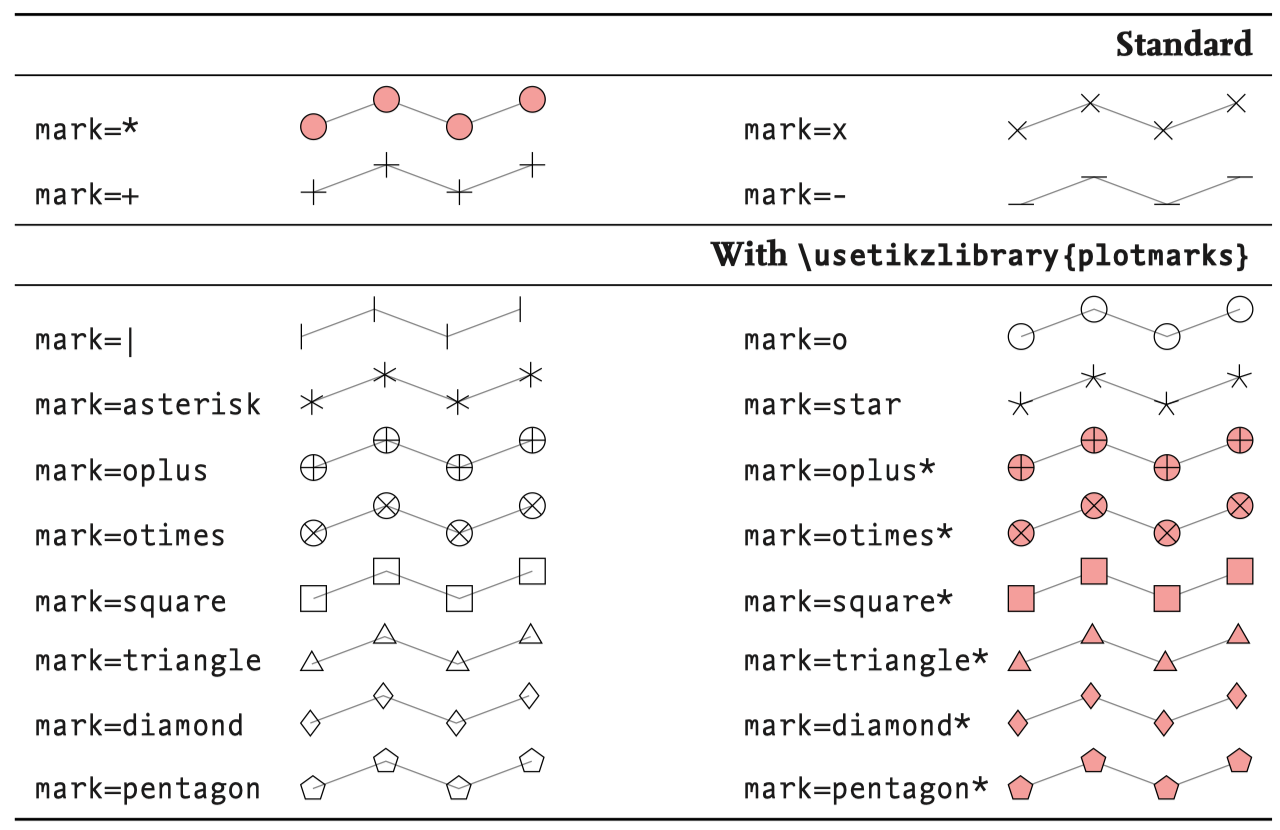
\includegraphics[width=0.7\textwidth]{pic/mark.png} 
% \end{figure}

\section{axis configure}
\textbf{enlargelimits=0.18} increases the default size of the axes \\ 
\textbf{curve} addplot+[sharp plot] ~~~ addplot+[smooth]       \\ 
\textbf{color} addplot[draw=black,fill=blue]\\ 
\textbf{title} title=Name\\ 
\textbf{legend} \\ 
\textit{position} legend style={[at={(.5,.5)}] | [legend pos=outer north east]} \\ 
\textit{columns} legend style={legend columns=[-1]|[2]}\\ 
\textit{align} legend cell align=[left] | [center] | [right]\\ 
\textbf{grid} xmajorgrids=true(|) ymajorgrids=true(-) grid=major(+)
\textbf{print number above bar}              
% nodes near coords, 
% nodes near coords align=vertical, 
% point meta=y * 1, % The displayed number. 

\section{Examples}
%------------饼图-------------

%------------柱状图------------
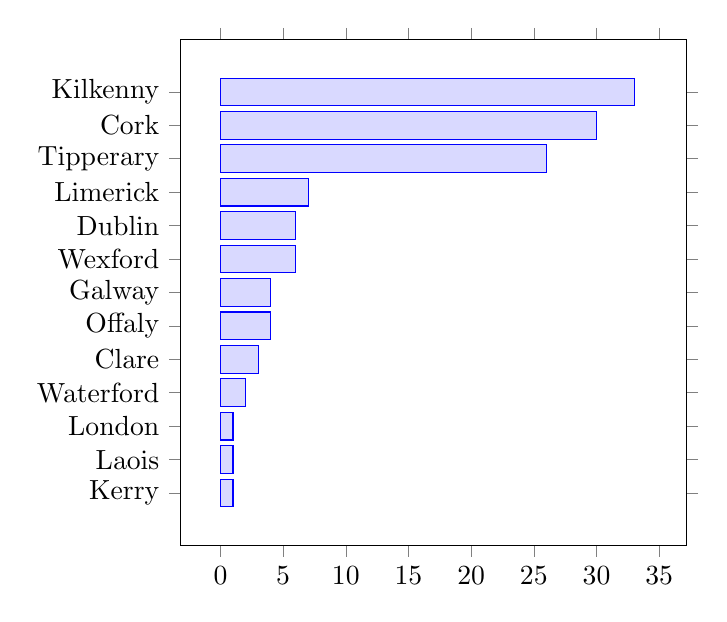
\begin{tikzpicture}
       \begin{axis}
              [xbar,width=8cm,height=8cm,bar width=10pt,enlargelimits=0.13,
              % nodes near coords, 
              % nodes near coords align=horizontal, 
              % point meta=x * 1, % The displayed number. 
              legend pos=south east, 
              % xlabel=\textbf{Frequency of Winning the Final}, 
              tick align=outside,
              xtick={0,5,...,35}, ytick={1,...,13},
              yticklabels={Kerry,Laois,London,Waterford,Clare,Offaly,Galway,Wexford,Dublin,Limerick,Tipperary,Cork,Kilkenny}] 
              \addplot[draw=blue, fill=blue!15] coordinates
              {(1,1) (1,2) (1,3) (2,4) (3,5) (4,6) (4,7) (6,8) (6,9) (7,10) (26,11) (30,12) (33,13)}; 
       \end{axis}
\end{tikzpicture}
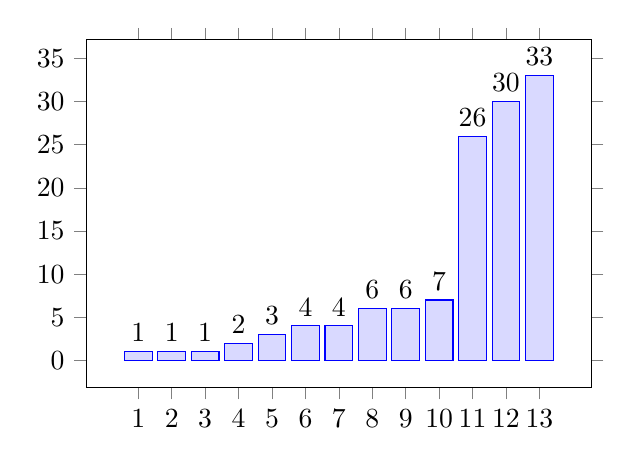
\begin{tikzpicture}
       \begin{axis}
              [ybar,width=8cm,height=6cm,bar width=10pt,enlargelimits=0.13,
              nodes near coords, 
              nodes near coords align=vertical, 
              point meta=y * 1, % The displayed number. 
              legend pos=south east, 
              % ylabel=\textbf{Frequency of Winning the Final}, 
              tick align=outside,
              ytick={0,5,...,35}, 
              xtick={1,...,13}
              % ,xticklabels={Kerry,Laois,London,Waterford,Clare,Offaly,Galway,Wexford,Dublin,Limerick,Tipperary,Cork,Kilkenny}
              ] 
              
              \addplot[draw=blue, fill=blue!15] 
                     coordinates {(1,1) (2,1) (3,1) (4,2) (5,3) (6,4) (7,4) (8,6) (9,6) (10,7) (11,26) (12,30) (13,33)}; 
       \end{axis}
\end{tikzpicture}

%------------分组--------------
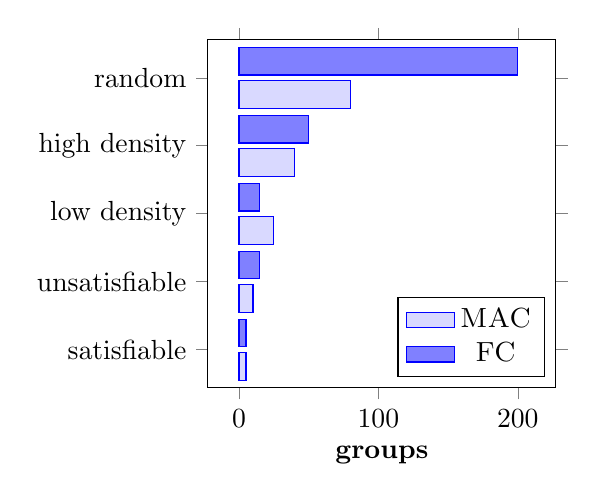
\begin{tikzpicture}
       \begin{axis} 
              [xbar,enlargelimits=0.14,width=6cm,height=6cm,, 
              bar width=10pt,area legend,legend pos=south east, 
              % legend style={legend pos=north east, cells={anchor=west}},
              tick align=outside,xlabel=\textbf{groups},
              ytick={1,...,5},
              yticklabels={satisfiable,unsatisfiable, low density,high density,random}] 
       \addplot[draw=blue,fill=blue!15]       
              coordinates {(5,1) (10,2) (25,3) (40,4) (80,5)}; 
       \addlegendentry{\textsc{MAC}} 
       \addplot[draw=blue,fill=blue!50]       
              coordinates {(5,1) (15,2) (15,3) (50,4) (200,5)}; 
       \addlegendentry{\textsc{FC}} 
       \end{axis}
\end{tikzpicture}
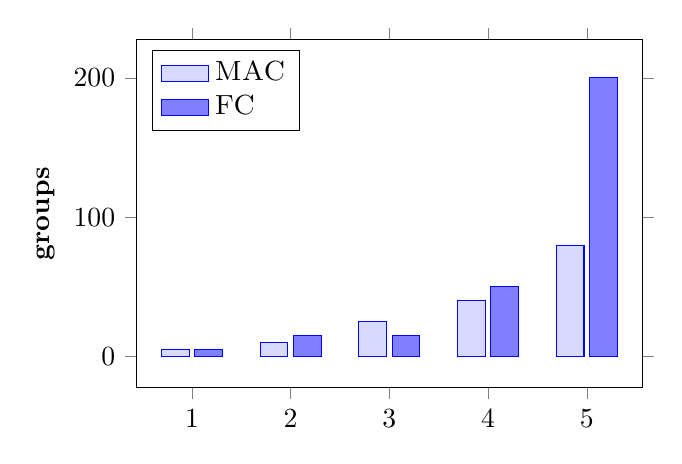
\begin{tikzpicture}
       \begin{axis} 
              [ybar,enlargelimits=0.14,width=8cm,height=6cm,, 
              bar width=10pt,area legend,legend pos=south east, 
              legend style={legend pos=north west, cells={anchor=west}},
              tick align=outside,
              ylabel=\textbf{groups},
              xtick={1,...,5}
              % ,xticklabels={satisfiable,unsatisfiable, low density,high density,random}
              ] 
       \addplot[draw=blue,fill=blue!15]       
              coordinates {(1,5) (2,10) (3,25) (4,40) (5,80)}; 
       \addlegendentry{\textsc{MAC}} 
       \addplot[draw=blue,fill=blue!50]       
              coordinates {(1,5) (2,15) (3,15) (4,50) (5,200)}; 
       \addlegendentry{\textsc{FC}} 
       \end{axis}
\end{tikzpicture}

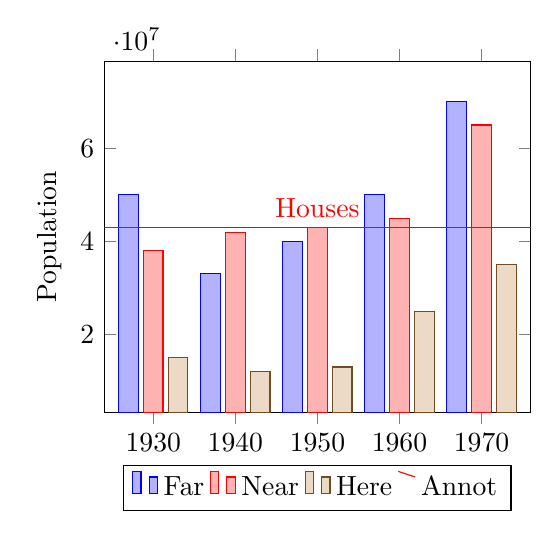
\begin{tikzpicture}
       \begin{axis}[
              x tick label style={
                     /pgf/number format/1000 sep=},
              ylabel=Population,
              enlargelimits=0.15,
              legend style={at={(0.5,-0.15)},
                     anchor=north,legend columns=-1},
              ybar,
              bar width=7pt,
       ]
       \addplot 
              coordinates {(1930,50e6) (1940,33e6)
                            (1950,40e6) (1960,50e6) (1970,70e6)};

       \addplot 
              coordinates {(1930,38e6) (1940,42e6) 
                     (1950,43e6) (1960,45e6) (1970,65e6)};

       \addplot 
              coordinates {(1930,15e6) (1940,12e6) 
                     (1950,13e6) (1960,25e6) (1970,35e6)};

       \addplot[red,sharp plot,update limits=false] 
              coordinates {(1910,4.3e7) (1990,4.3e7)} 
              node[above] at (axis cs:1950,4.3e7) {Houses};

       \legend{Far,Near,Here,Annot}
       \end{axis}
\end{tikzpicture}

%------------breakdown--------
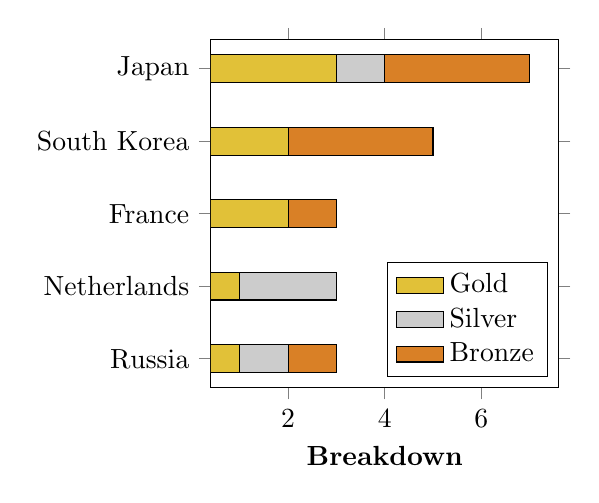
\begin{tikzpicture}
       \begin{axis} 
              [xbar stacked, stack plots=x, tick align=outside, 
              width=6cm, height=6cm, bar width=10pt, 
              legend style={legend pos=south east, cells={anchor=west}}, area legend, 
              xlabel=\textbf{Breakdown}, 
              ytick={1,...,5}, 
              yticklabels={Russia,Netherlands,France, South Korea,Japan}] 
              \addplot[draw=black,fill=yellow!50!brown]
                     coordinates {(1,1) (1,2) (2,3) (2,4) (3,5)}; 
              \addlegendentry{Gold} 
              \addplot[draw=black,fill=white!60!gray]
                     coordinates {(1,1) (2,2) (0,3) (0,4) (1,5)}; 
              \addlegendentry{Silver} 
              \addplot[draw=black,fill=orange!70!gray]
                     coordinates {(1,1) (0,2) (1,3) (3,4) (3,5)}; 
              \addlegendentry{Bronze} 
       \end{axis}
\end{tikzpicture}
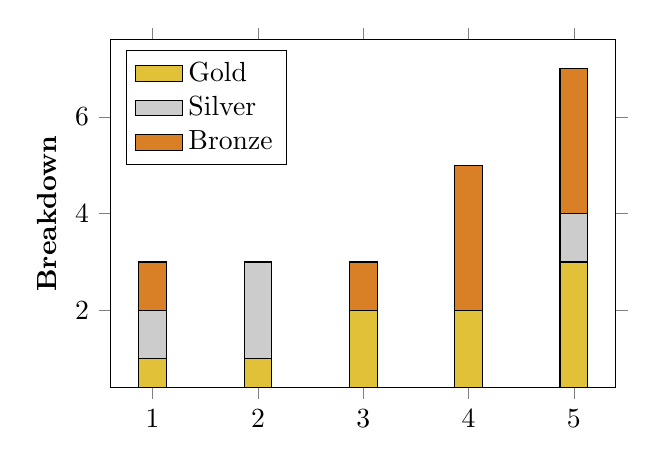
\begin{tikzpicture}
       \begin{axis} 
              [ybar stacked, stack plots=y, tick align=outside, 
              width=8cm, height=6cm, bar width=10pt, 
              legend style={legend pos=north west, cells={anchor=west}}, area legend, 
              ylabel=\textbf{Breakdown}, 
              xtick={1,...,5} 
              % ,xticklabels={Russia,Netherlands,France, South Korea,Japan}
              ] 
              \addplot[draw=black,fill=yellow!50!brown]
                     coordinates {(1,1) (2,1) (3,2) (4,2) (5,3)}; 
              \addlegendentry{Gold} 
              \addplot[draw=black,fill=white!60!gray]
                     coordinates {(1,1) (2,2) (3,0) (4,0) (5,1)}; 
              \addlegendentry{Silver} 
              \addplot[draw=black,fill=orange!70!gray]
                     coordinates {(1,1) (2,0) (3,1) (4,3) (5,3)}; 
              \addlegendentry{Bronze} 
       \end{axis}
\end{tikzpicture}

%-----------折线图-------------
\begin{tikzpicture}      
       \begin{axis}
              [width=\textwidth, height=13cm, enlargelimits=0.13,tick align=outside, 
              legend style={cells={anchor=west},legend pos=north east}, 
              xticklabels={Jan,Feb,Mar,Apr,May,Jun,Jul,Aug,Sep,Oct,Nov,Dec}, 
              xtick={1,2,3,4,5,6,7,8,9,10,11,12},
              xlabel=\textbf{Month}, ylabel=\textbf{Rainfall}]
              
              \node[coordinate,pin=above:{Very Wet}] at (axis cs:1,223.9) {}; 
              \node[coordinate,pin=right:{Very Dry}] at (axis cs:2,14.7) {}; 
              
              % \addplot+[sharp plot] 
                     % coordinates {(1,171.5) (2,116.4) (3,157.4) (4,67.7) (5,40.2) (6,127.6) (7,44.3) (8,192.1) (9,112.4) (10,177.5) (11,136.2) (12,94.8)}; 
              \addplot table[col sep=comma] {data.csv};
              \addlegendentry{Belmullet}

              \addplot+[sharp plot] 
                     coordinates {(1,135.5) (2,30.8) (3,97.3) (4,28.6) (5,19.2) (6,90.2) (7,100.6) (8,171.6) (9,81.8) (10,121.0) (11,77.0) (12,63.7)}; 
              \addlegendentry{Birr} 

              \addplot+[sharp plot] 
                     coordinates {(1,195.1) (2,49.8) (3,113.5) (4,53.7) (5,75.6) (6,138.5) (7,148.1) (8,163.6) (9,123.8) (10,139.2) (11,79.4) (12,60.2)}; 
              \addlegendentry{Cork Airport} 
              
              \addplot+[sharp plot] 
                     coordinates {(1,96.9) (2,14.7) (3,102.4) (4,27.0) (5,32.7) (6,76.4) (7,111.5) (8,192.4) (9,111.8) (10,97.4) (11,39.6) (12,39.5)}; 
              \addlegendentry{Dublin Airport} 
              
              \addplot+[smooth] 
                     coordinates {(1,223.9) (2,58.0) (3,102.9) (4,49.2) (5,35.9) (6,110.8) (7,100.8) (8,176.6) (9,86.4) (10,156.4) (11,92.2) (12,75.1)}; 
              \addlegendentry{Shannon Airport} 

              \addplot+[only marks, mark=x, draw=blue] 
                     coordinates {(1,1) (2,1) (3,1) (4,1) (5,1) (6,11) (7,1) (8,1) (9,1) (10,1) (11,1) (12,1)}; 
              
       \end{axis}
\end{tikzpicture}

%-----------数据格式-----------
% \begin{filecontents}{A.dat}
% 0 0
% 1 1
% 2 2
% \end{filecontents}

% \begin{filecontents}{B.csv}
% a,b,c
% 0,1,1
% 1,2,3
% 2,3,2
% \end{filecontents}

% \begin{filecontents}{C.montypython}
% foo bar baz
% 0 2 3
% 1 3 4
% 2 4 5
% \end{filecontents}

\begin{tikzpicture}
       \begin{axis}
       \addplot table {data/A.dat};
       \addplot table[col sep=comma, x=a, y=c] {data/B.csv};
       \addplot table[x=foo, y=bar] {data/C.montypython};
       \addplot table[x index=0, y index=2] {data/C.montypython};

       \legend{A,B,C1,C2}
       \end{axis}
\end{tikzpicture}
%------------------线性回归--------------------
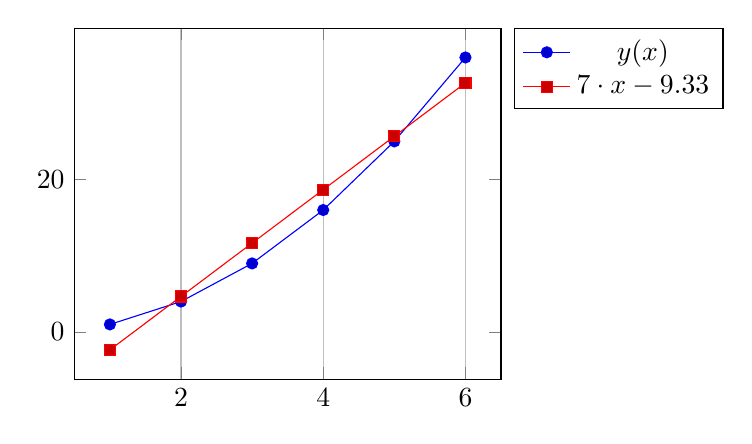
\begin{tikzpicture}
       \begin{axis}[xmajorgrids=true, legend pos=outer north east] % 将图例放在图外,位于图的东北角
       \addplot 
       table                               % 绘制原始数据的折线图
       {           		                % X,Y的原始数据
        X Y
        1 1
        2 4
        3 9
        4 16 
        5 25
        6 36
       };
       \addplot
       table[y={create col/linear regression={y=Y}}] % 对输入的数据作线性回归
       {   				
        X Y
        1 1
        2 4
        3 9
        4 16 
        5 25
        6 36
       };
       \addlegendentry{$y(x)$}          % 给第一个图像添加图例,即原始函数y(x)
       \addlegendentry{                 % 给第二个图像添加图例,即线性回归结果a*x+b
       $\pgfmathprintnumber{\pgfplotstableregressiona} \cdot x
       \pgfmathprintnumber[print sign]{\pgfplotstableregressionb}$}
       \end{axis}
\end{tikzpicture}
%------------------折线+柱状--------------------
\begin{tikzpicture}
       \begin{axis}
              [width=12cm,height=6cm,bar width=10pt,enlargelimits=0.13,
              legend pos=south east, 
              tick align=outside,
              xtick={1,...,12}
              ] 
              
              \addplot[ybar,draw=blue, fill=blue!15] table[col sep=comma, x index=0, y index=1] {data.csv};
              % \addplot+[only marks] table[col sep=comma, x index=0, y index=2] {data.csv};
              % \addplot+[smooth, fill opacity=0] table[col sep=comma, x index=0, y index=2] {data.csv};
              \addplot+[sharp plot] table[col sep=comma, x index=0, y index=2] {data.csv};
       \end{axis}
\end{tikzpicture}

%------------------放大局部--\usetikzlibrary{spy}--
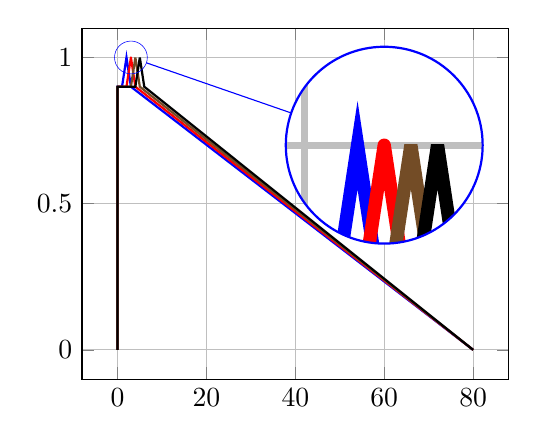
\begin{tikzpicture}[spy using outlines= {circle, magnification=6, connect spies}] 
       \begin{axis}[no markers,grid=major, every axis plot post/.append style={thick}]
       \addplot coordinates {(0, 0) (0, 0.9) (1, 0.9) (2, 1) (3, 0.9) (80, 0)}; 
       \addplot+ [line join=round] coordinates {(0, 0) (0, 0.9) (2, 0.9) (3, 1) (4, 0.9) (80, 0)}; 
       \addplot+ [line join=bevel] coordinates {(0, 0) (0, 0.9) (3, 0.9) (4, 1) (5, 0.9) (80, 0)}; 
       \addplot+ [miter limit=5] coordinates {(0, 0) (0, 0.9) (4, 0.9) (5, 1) (6, 0.9) (80, 0)};
       \coordinate (spypoint) at (3,1); 
       \coordinate (magnifyglass) at (60,0.7); 
\end{axis}
\spy [blue, size=2.5cm] on (spypoint) in node[fill=white] at (magnifyglass); 
\end{tikzpicture}

%------------------框选局部--\usepgfplotslibrary{groupplots}--------------------
\begin{tikzpicture}
\begin{groupplot}[group style={group size=3 by 1},xmin=0,ymin=0,height=4cm,width=5cm,no markers]
       \nextgroupplot
       \addplot[very thick] file {data/group-1.dat};
       \draw[red,dashed,thick] (axis cs:0,0) rectangle (axis cs:5,30);
       \nextgroupplot[xmax=5,ymax=30]
       \addplot[very thick] file {data/group-1.dat};
       \draw[red,dashed,thick] (axis cs:3,10) rectangle (axis cs:5,25);
       \nextgroupplot[xmin=3,xmax=5,ymin=10,ymax=25]
       \addplot[very thick] file {data/group-1.dat};
\end{groupplot}
\draw[thick,blue,->,shorten >=2pt,shorten <=2pt] 
              (group c1r1.east) -- (group c2r1.west);
\draw[thick,blue,->,shorten >=2pt,shorten <=2pt] 
              (group c2r1.east) -- (group c3r1.west);
\end{tikzpicture}

%------------------面积图-------------------------
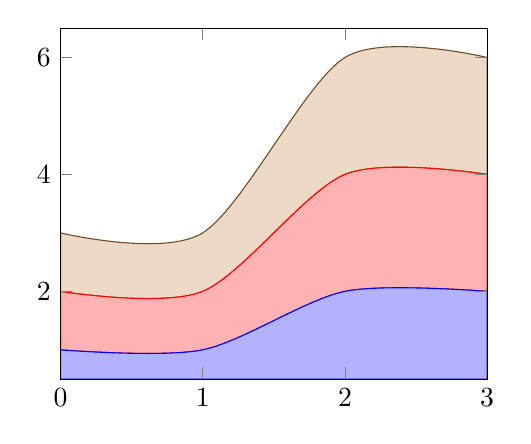
\begin{tikzpicture}
	\begin{axis}[
		smooth,
		stack plots=y,
		area style,
		enlarge x limits=false]
	\addplot coordinates
		{(0,1) (1,1) (2,2) (3,2)} 
		\closedcycle;
	\addplot coordinates
		{(0,1) (1,1) (2,2) (3,2)}
		\closedcycle;
	\addplot coordinates
		{(0,1) (1,1) (2,2) (3,2)}
		\closedcycle;
	\end{axis}
\end{tikzpicture}
%------------------折叠坐标轴----------------------
\begin{tikzpicture} 
       \begin{axis}[ 
              axis x line=bottom, axis y line=center, 
              tick align=outside, 
              axis y discontinuity=crunch, ymin=95, 
              enlargelimits=false, ] 
              \addplot [blue,mark=none, domain=-4:4,samples=20, ] {x*x+x+104}; 
       \end{axis} 
\end{tikzpicture}

%------------------Log10--------------------------
% \pgfplotsset{every axis/.append style={ font=\footnotesize, thin, tick style={ultra thin}}, }
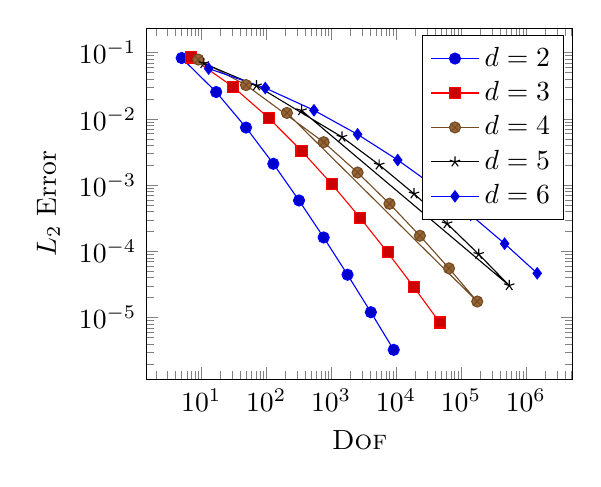
\begin{tikzpicture} \begin{loglogaxis}[ xlabel=\textsc{Dof}, ylabel=$L_2$ Error ] 
    \addplot coordinates {(5,8.312e-02) (17,2.547e-02) (49,7.407e-03) (129,2.102e-03) (321,5.874e-04) (769,1.623e-04) (1793,4.442e-05) (4097,1.207e-05) (9217,3.261e-06) };
    \addplot coordinates {(7,8.472e-02) (31,3.044e-02) (111,1.022e-02) (351,3.303e-03) (1023,1.039e-03) (2815,3.196e-04) (7423,9.658e-05) (18943,2.873e-05) (47103,8.437e-06) };
    \addplot coordinates {(9,7.881e-02) (49,3.243e-02) (769,4.454e-03) (2561,1.551e-03) (7937,5.236e-04) (23297,1.723e-04) (65537,5.545e-05) (178177,1.751e-05) (209,1.232e-02) };
    \addplot coordinates {(11,6.887e-02) (71,3.177e-02) (1471,5.334e-03) (5503,2.027e-03) (18943,7.415e-04) (61183,2.628e-04) (187903,9.063e-05) (553983,3.053e-05) (351,1.341e-02) };
    \addplot coordinates {(13,5.755e-02) (97,2.925e-02) (545,1.351e-02) (2561,5.842e-03) (10625,2.397e-03) (40193,9.414e-04) (141569,3.564e-04) (471041,1.308e-04) (1496065,4.670e-05) }; 
    % \plotcoords 
    \legend{$d=2$,$d=3$,$d=4$,$d=5$,$d=6$} 
\end{loglogaxis} 
\end{tikzpicture}

%-----------------热度图--------------------------
\pgfplotsset{footnotesize,samples=10, domain=0:1,point meta min=0, point meta max=1} 
\begin{center}% note that \centering uses less vspace... 
       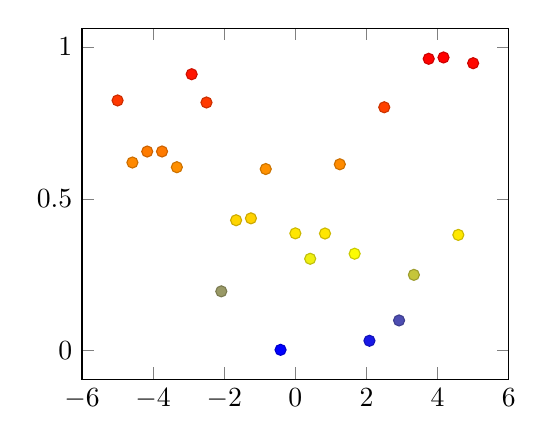
\begin{tikzpicture} 
              \begin{axis}[colorbar,colorbar horizontal,colorbar to name={storedcolorbar}] 
                     \addplot [scatter,only marks,mark=*] {rnd}; 
              \end{axis} 
       \end{tikzpicture} % 
       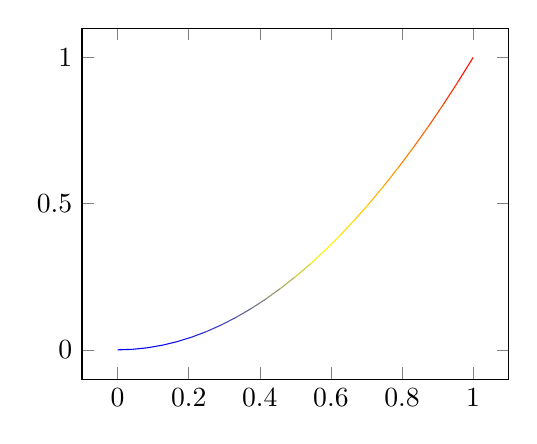
\begin{tikzpicture} 
              \begin{axis} 
                     \addplot+ [domain=0:1,mark=none,mesh] {x^2}; 
              \end{axis} 
       \end{tikzpicture} % 
       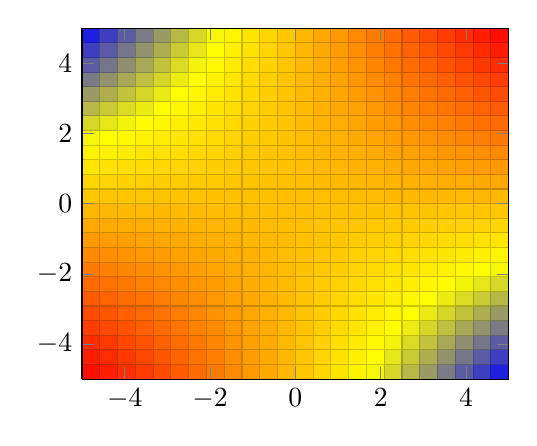
\begin{tikzpicture} 
                     \begin{axis}[view={0}{90}] \addplot3 [surf] {x*y}; 
                     \end{axis} 
       \end{tikzpicture} \\
\end{center}


\end{document}

